\begin{figure}[ht]
\centering
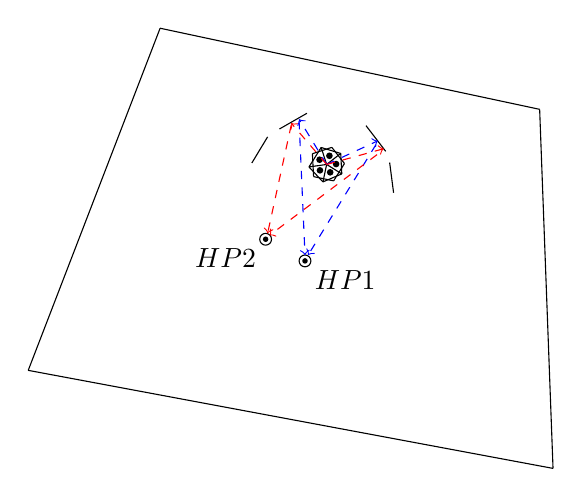
\begin{tikzpicture}[scale = 0.5]
% KOORDINATEN
% \coordinate[label=below:$\texttt{Ursprung}$] (Ursprung) at (0,0);
\coordinate (POSIKO) at (.7,1.7);
\coordinate[label=below right:$\text{\small HP1}$]  (HP1) at (.15,-.75);
\coordinate[label=below left:$\text{\small HP2}$]  (HP2) at (-.85,-.2);

% Raum
\coordinate (LO) at (-3.53,5.16);
\coordinate (RO) at (6.11,3.10);
\coordinate (LU) at (-6.88,-3.53);
\coordinate (RU) at (6.45,-6.02);
% Reflektor 1
\coordinate (R1U) at (-1.2,1.737);
\coordinate (R1O) at (-.8,2.4);
% Reflektor 2
\coordinate (R2U) at (-.5,2.6);
\coordinate (R2O) at (0.2,3);
% Reflektor 3
\coordinate (R3U) at (2.2,2.033);
\coordinate (R3O) at (1.7,2.685);
% Reflektor 4
\coordinate (R4O) at (2.3,1.749);
\coordinate (R4U) at (2.4,.981);
% IKO
\coordinate (IKO1) at (.25126,1.6369);
\coordinate (IKO2) at (0.60578,1.2567);
\coordinate (IKO3) at (1.0843,1.4599);
\coordinate (IKO4) at (1.0571,1.979 );
\coordinate (IKO5) at (0.55997,2.131);
\coordinate (IKO6) at (0.36858,1.3909);
\coordinate (IKO7) at (0.87706,1.2829);
\coordinate (IKO8) at (1.1525,1.7237);
\coordinate (IKO9) at ( 0.83249,2.1334);
\coordinate (IKO10) at ( 0.3381,1.9727);

% ZEICHNEN
\draw (R1U) -- (R1O);
\draw (R2U) -- (R2O);
\draw (R3U) -- (R3O);
\draw (R4U) -- (R4O);

\draw (IKO6) -- (IKO7);
\draw (IKO7) -- (IKO8);
\draw (IKO8) -- (IKO9);
\draw (IKO9) -- (IKO10);
\draw (IKO10) -- (IKO6);

\draw (IKO1) -- (IKO2);
\draw (IKO2) -- (IKO3);
\draw (IKO3) -- (IKO4);
\draw (IKO4) -- (IKO5);
\draw (IKO5) -- (IKO1);

\draw (POSIKO) -- (IKO1);
\draw (POSIKO) -- (IKO2);
\draw (POSIKO) -- (IKO3);
\draw (POSIKO) -- (IKO4);
\draw (POSIKO) -- (IKO5);

\draw (LO) -- (RO);
\draw (RO) -- (RU);
\draw (RU) -- (LU);
\draw (LU) -- (LO);

% \draw[help lines] (-3,-3) grid (3,3);
\draw (HP1) circle [radius=1.5mm] ;
\draw (HP2) circle [radius=1.5mm] ;

% \fill (Ursprung) circle (2pt);
\fill (POSIKO) circle (1pt);
\fill (.79,1.5) circle (2.4pt);
\fill (.94,1.71) circle (2.4pt);
\fill (.77,1.92) circle (2.4pt);
\fill (.52,1.82) circle (2.4pt);
\fill (.53,1.55) circle (2.4pt);
\fill (HP1) circle (2pt);
\fill (HP2) circle (2pt);

% Schallstrahl links HP1
% \draw[blue,dashed,->,-triangle 90,fill=blue] (POSIKO) -- (0,2.85);
\draw[blue,dashed,->] (POSIKO) -- (0,2.85);
\draw[blue,dashed,->] (0,2.8) -- (.15,-.6);
% Schallstrahl rechts HP1
\draw[blue,dashed,->] (POSIKO) -- (2,2.3);
\draw[blue,dashed,->] (1.95,2.20) -- (.23,-.6);
% Schallstrahl links HP2
\draw[red,dashed,->] (POSIKO) -- (-.2,2.75);
\draw[red,dashed,->] (-.2,2.7) -- (-.8,-.05);
% Schallstrahl rechts HP2
\draw[red,dashed,->] (POSIKO) -- (2.15,2.1);
\draw[red,dashed,->] (1.98,1.95) -- (-0.75,-.1);
\end{tikzpicture}
\caption{Diagram of the CUBE for the listening experiment. The hearing position 1 (HP1) was directly in front of the IKO with a distance of $2.5m$. The hearing position 2 (HP2) was further ahead and approximatley 1 meter apart. The reflectors were placed symmetrically around the IKO. The noise and the beamformed sounds were presented by the IKO.}
\end{figure}